\documentclass[12pt]{article}
\usepackage[utf8]{inputenc}
\usepackage[russian]{babel}
\usepackage{graphicx}
\usepackage{array}
\usepackage[a4paper, left=1cm, right=1cm, top=1.27cm, bottom=1.27cm]{geometry}
\usepackage{setspace}
\usepackage{tabularx}
\usepackage{makecell}
\usepackage{longtable}
\usepackage{multirow}
\usepackage{caption}
\onehalfspacing


\begin{document}


\begin{table}[h]
    \centering
    \renewcommand{\arraystretch}{1.5} % Увеличиваем межстрочный интервал
    \begin{tabular}{|m{11cm}|m{6cm}|} % Первая колонка шире, вторая для лого
        \hline
        \begin{center}
            \textbf{Университет ITMO}\\
            \textbf{Физико-технический мегафакультет}\\
            \textbf{Физический факультет}
        \end{center} 
        & 
        \begin{center}
            
\includegraphics[height=1.3cm]{logo.jpg}
        \end{center} \\
        \hline
    \end{tabular}
\end{table}

\noindent\makebox[\linewidth]{\rule{\textwidth}{2pt}}

\vspace{10pt}

\begin{table}[h]
    \centering
    \renewcommand{\arraystretch}{1.7}
    \begin{tabular}{|p{4cm}p{4cm}|p{8cm}|}
        \hline
        Группа N3150 & & К работе допущен \underline{\hspace{4cm}} \\
        \hline
        Студенты & \hfill \multirow[0pt]{3}{*}{\makecell[c]{Пахомов В.Ю \\ Фармахини Ф.Р. \\ Петров Д.О}}  & Работа выполнена \underline{\hspace{4cm}} \\
        & & \\
        & & \\
        \hline
        \multicolumn{2}{|c|}{Преподаватель \underline{\hspace{5cm}}}  & Отчет принят \underline{\hspace{5cm}} \\
        \hline
    \end{tabular}
\end{table}

\begin{center}
    \fontsize{20pt}{21.5pt} \selectfont
    \textbf{Рабочий протокол и отчет по}\\
    \textbf{лабораторной работе № 1.01}
\end{center}

\noindent\makebox[\linewidth]{\rule{\textwidth}{1pt}}
\noindent\makebox[\linewidth]{\rule{\textwidth}{1pt}}

\begin{flushleft}
    1. Цель работы.\\
    Исследование распределения случайной величины на примере
    многократных измерений определённого интервала времени.
\end{flushleft}

\begin{flushleft}
    2. Задачи, решаемые при выполнении работы.\\
    \hspace{0.63cm} 1. Провести многократные измерения определенного интервала времени.\\
    \hspace{0.63cm} 2. Построить гистограмму распределения результатов измерения.\\
    \hspace{0.63cm} 3. Вычислить среднее значение и дисперсию полученной выборки.\\
    \hspace{0.63cm} 4. Сравнить гистограмму с графиком функции Гаусса с такими.\\
    \hspace{0.63cm} же как и у экспериментального распределения средним значением и дисперсией.\\
\end{flushleft}

\begin{flushleft}
    3. Объект исследования. \\
    Распределение случайной величины, полученной в результате многократных измерений заданного промежутка времени. \\
\end{flushleft}

\begin{flushleft}
    4. Метод экспериментального исследования. \\
    Экспериментальный метод включает в себя многократное измерение определенного 
    временного интервала с помощью цифрового секундомера, построение гистограммы 
    распределения полученных значений, вычисление статистических параметров 
    (среднего значения, дисперсии) и сравнение полученного распределения с 
    нормальным (гауссовским). \\
\end{flushleft}

\begin{flushleft}
    5. Рабочие формулы и исходные данные. \\
    \hspace{0.63cm} 1. Выборочное значение среднего: $ \langle t \rangle _N = \frac{1}{N} \sum_{i=1}^{N}t_i $ \\
    \hspace{0.63cm} 2. Выборочное среднеквадратичное отклонение: $ \sigma_N = \sqrt{\frac{1}{N-1} \sum_{i=1}^{N} (t_i - \langle t \rangle_N)^2} $ \\
    \hspace{0.63cm} 3. Плотность вероятности нормального распределения: $ \rho(t) = \frac{1}{\sigma\sqrt{2\pi}} exp (-\frac{(t - \langle t \rangle)^2}{2 \sigma^2})$ \\
\end{flushleft}

\newpage

\begin{flushleft}
    6. Измерительные приборы.
\end{flushleft}

\begin{table}[h]
    \centering
    \renewcommand{\arraystretch}{1.5}
    {\itshape
    \begin{tabular}{|c|c|c|c|c|}
        \hline
        № п/п & Наименование & Тип прибора & Используемый диапазон & Погрешность прибора\\
        \hline
        1 & Секундомер & Электронный & 0-60 с & ±0.01 с\\
        \hline
    \end{tabular}
    }
\end{table}

\begin{flushleft}
    7. Схема установки.
\end{flushleft}

\begin{flushleft}
    8. Результаты прямых измерений и их обработки.
\end{flushleft}

\begin{longtable}{|c|c|c|c|}
    \captionsetup{justification=centering, font=bf}
    \caption{Результаты прямых измерений} \\
    \hline
    № & $t_i, \ c$ & $t_i - \langle t \rangle_N, \ c$ & $(t_i - \langle t \rangle_N)^2, \ c^2$ \\
    \hline
    \endfirsthead
    
    \hline
    № & $t_i, \ c$ & $t_i - \langle t \rangle_N, \ c$ & $(t_i - \langle t \rangle_N)^2, \ c^2$ \\
    \hline
    \endhead

    \hline
    \endfoot
    
    \hline
    \endlastfoot
    
    1	&	4.87	&	-0.16	&	0.03	\\
    \hline
    2	&	5.07	&	0.04	&	0	\\
    \hline
    3	&	4.65	&	-0.38	&	0.14	\\
    \hline
    4	&	5.15	&	0.12	&	0.01	\\
    \hline
    5	&	5.17	&	0.14	&	0.02	\\
    \hline
    6	&	5.11	&	0.08	&	0.01	\\
    \hline
    7	&	4.86	&	-0.17	&	0.03	\\
    \hline
    8	&	4.76	&	-0.27	&	0.07	\\
    \hline
    9	&	5.34	&	0.31	&	0.1	\\
    \hline
    10	&	4.49	&	-0.54	&	0.29	\\
    \hline
    11	&	5.31	&	0.28	&	0.08	\\
    \hline
    12	&	4.72	&	-0.31	&	0.1	\\
    \hline
    13	&	5.47	&	0.44	&	0.19	\\
    \hline
    14	&	4.67	&	-0.36	&	0.13	\\
    \hline
    15	&	5.42	&	0.39	&	0.15	\\
    \hline
    16	&	5.74	&	0.71	&	0.5	\\
    \hline
    17	&	5.13	&	0.1	&	0.01	\\
    \hline
    18	&	5.41	&	0.38	&	0.14	\\
    \hline
    19	&	4.84	&	-0.19	&	0.04	\\
    \hline
    20	&	4.91	&	-0.12	&	0.01	\\
    \hline
    21	&	5.4	&	0.37	&	0.14	\\
    \hline
    22	&	5.34	&	0.31	&	0.1	\\
    \hline
    23	&	4.79	&	-0.24	&	0.06	\\
    \hline
    24	&	4.8	&	-0.23	&	0.05	\\
    \hline
    25	&	4.83	&	-0.2	&	0.04	\\
    \hline
    26	&	5.17	&	0.14	&	0.02	\\
    \hline
    27	&	5.07	&	0.04	&	0	\\
    \hline
    28	&	5.03	&	0	&	0	\\
    \hline
    29	&	4.89	&	-0.14	&	0.02	\\
    \hline
    30	&	4.92	&	-0.11	&	0.01	\\
    \hline
    31	&	5.13	&	0.1	&	0.01	\\
    \hline
    32	&	5.06	&	0.03	&	0	\\
    \hline
    33	&	4.79	&	-0.24	&	0.06	\\
    \hline
    34	&	5.07	&	0.04	&	0	\\
    \hline
    35	&	4.92	&	-0.11	&	0.01	\\
    \hline
    36	&	5.23	&	0.2	&	0.04	\\
    \hline
    37	&	4.97	&	-0.06	&	0	\\
    \hline
    38	&	5.13	&	0.1	&	0.01	\\
    \hline
    39	&	5.18	&	0.15	&	0.02	\\
    \hline
    40	&	4.87	&	-0.16	&	0.03	\\
    \hline
    41	&	5.05	&	0.02	&	0	\\
    \hline
    42	&	4.74	&	-0.29	&	0.08	\\
    \hline
    43	&	4.92	&	-0.11	&	0.01	\\
    \hline
    44	&	5.22	&	0.19	&	0.04	\\
    \hline
    45	&	5.06	&	0.03	&	0	\\
    \hline
    46	&	4.94	&	-0.09	&	0.01	\\
    \hline
    47	&	5.03	&	0	&	0	\\
    \hline
    48	&	5.02	&	-0.01	&	0	\\
    \hline
    49	&	4.98	&	-0.05	&	0	\\
    \hline
    50	&	4.92	&	-0.11	&	0.01	\\
    \hline
    
    \hline
    & $\langle t \rangle_N = 5.031 \ c$ & 
    $\sum\limits_{i=1}^{N} (t_i - \langle t \rangle_N) = 0.06 \ c$ & 
    \makecell{$\sigma_N = 0.238 \ c$ \\ $\rho_{\max} = 1.7 \ c^{-1}$} \\
\end{longtable}

\begin{flushleft}
    9. Расчет результатов косвенных измерений (таблицы, примеры расчетов).
\end{flushleft}

\begin{flushleft}
    Наименьший и наибольший t: \\
    $ t_{min} = 4.49 $ \\
    $ t_{max} = 5.74 $ \\
    Количество промежутков m равно: $ \sqrt{N} \approx 7 $ \\
    Вычисление промежутка: $ \Delta t = \frac{t_{max} - t_{min}}{m} \approx 0.18 = 0.2 $ \\
    Формула для вычисления плотности вероятности: $ \rho_i = \frac{\Delta N}{N \Delta t} $ \\
    Выборочное значение среднего: $ \langle t \rangle _N = \frac{1}{N} \sum_{i=1}^{N}t_i \approx 5.031 $ \\
    Выборочное среднеквадратичное отклонение: $ \sigma_N = \sqrt{\frac{1}{N-1} \sum_{i=1}^{N} (t_i - \langle t \rangle_N)^2} \approx 0.238 $ \\
    Максимальное значение плотности распределения: $ \rho_{max} = \frac{1}{\sigma\sqrt{2\pi}} \approx 1.7 $ \\
    Cреднеквадратичное отклонение среднего значения: $ \sigma_{\langle t \rangle} = \sqrt{\frac{1}{N (N - 1)} \sum_{i=1}^{N} (t_i - \langle t \rangle_N)^2} \approx 0.034 $ \\
    Табличное значение коэффицента Стьюдента: $ t_{0.95,49} \approx 2.009 $ \\
    Доверительный интервал: $ \Delta t = t_{0.95,49} \cdot \sigma_{\langle t \rangle} \approx 0.0683 $ \\
\end{flushleft}

\begin{table}[h]
    \centering
    \captionsetup{justification=centering, font=bf}
    \caption{Данные для построения гистограммы}
    \renewcommand{\arraystretch}{1.5}
    \begin{tabular}{|c|c|c|c|c|}
        \hline
        \multirow{2}{*}{\makecell{Границы \\ интервалов, $c$}} & 
        \multirow{2}{*}{$\Delta N$} & 
        \multirow{2}{*}{$\frac{\Delta N}{N \Delta t}, \ c^{-1}$} & 
        \multirow{2}{*}{$t, \ c$} & 
        \multirow{2}{*}{$\rho, \ c^{-1}$} \\
        & & & & \\
        \hline
        [4.4; 4.6] & 1 & 0.1 & 4.5 & 0.139 \\
        \hline
        [4.6; 4.8] & 7 & 0.7 & 4.7 & 0.637 \\
        \hline
        [4.8; 5.0] & 15 & 1.5 & 4.9 & 1.439 \\
        \hline
        [5.0; 5.2] & 17 & 1.7 & 5.1 & 1.606 \\
        \hline
        [5.2; 5.4] & 5 & 0.5 & 5.3 & 0.886 \\
        \hline
        [5.4; 5.6] & 4 & 0.4 & 5.5 & 0.241 \\
        \hline
        [5.6; 5.8] & 1 & 0.1 & 5.7 & 0.033 \\
        \hline
    \end{tabular}
\end{table}

\begin{table}[h]
    \centering
    \captionsetup{justification=centering, font=bf}
    \caption{Стандартные доверительные интервалы}
    \renewcommand{\arraystretch}{1.5}
    \begin{tabular}{|c|c|c|c|c|c|}
        \hline
        & \multicolumn{2}{c|}{Интервал, $c$} & $\Delta N$ & $\frac{\Delta N}{N}$ & $P$ \\
        \cline{2-3}
        & от & до & & & \\
        \hline
        $\langle t \rangle_N \pm \sigma_N$ & 4.793 & 5.269 & 34 & 0.68 & 0.6827 \\
        \hline
        $\langle t \rangle_N \pm 2\sigma_N$ & 4.555 & 5.508 & 48 & 0.96 & 0.9545 \\  
        \hline
        $\langle t \rangle_N \pm 3\sigma_N$ & 4.317 & 5.746 & 50 & 1.00 & 0.9973 \\ 
        \hline
    \end{tabular}
\end{table}

\newpage

\begin{flushleft}
    10. Расчет погрешностей измерений (для прямых и косвенных измерений). \\
    Aбсолютная погрешность: $ \Delta x = | x - x_0 | = | 5.05 - 5 | = 0.05 $ \\
    Относительная погрешность: $ \epsilon = \frac{\Delta x}{x_0} = \frac{5.05}{5} = 0.01 $ \\
    Точность: $ t = \frac{1}{\epsilon} = \frac{1}{0.01} = 100 $ \\
\end{flushleft}

\begin{flushleft}
    11. Графики (перечень графиков, которые составляют Приложение 2). \\
    \begin{center}
        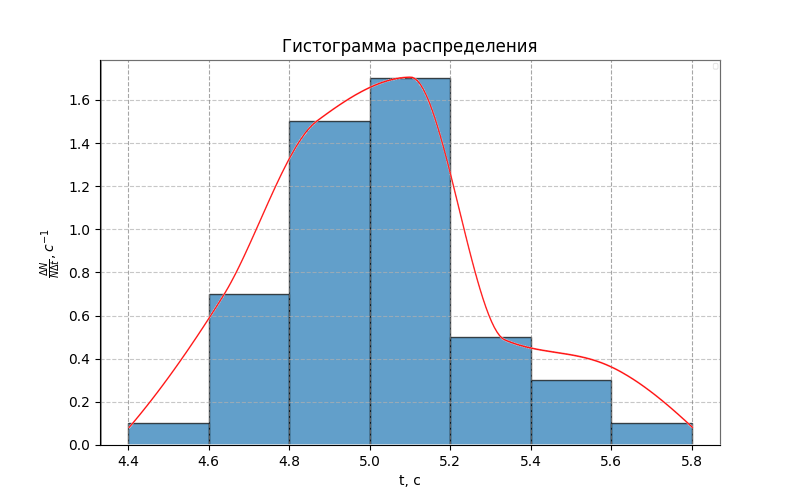
\includegraphics[height=9cm]{gistogram.png}
    \end{center}
\end{flushleft}

\begin{flushleft}
    12. Окончательные результаты. \\
    \hspace{0.63cm}Полученное математическое ожидание на основе измерений: \\
    \hspace{0.63cm}Aбсолютная погрешность: $ \Delta x = 0.05 $ \\
    \hspace{0.63cm}Относительная погрешность: $ \epsilon = 0.01 $ \\
    \hspace{0.63cm}Доверительный интервал: $ \Delta t = 0.0683 $ \\
\end{flushleft}

\begin{flushleft}
    13. Выводы и анализ результатов работы. \\
    В ходе выполнения лабораторной работы был изучен и применен закон нормального распределения путем проведения
    многократных измерений времени с помощью электронного секундомера. Это позволило оценить качество
    полученных данных и характер их распределения. Были вычисленны следующие величины:
    \begin{itemize}
        \item Максимальная плотность распределения
        \item Среднее арифметическое всех результатов измерений
        \item Среднеквадратичное отклонение среднего значения
        \item Доверительный интервал
    \end{itemize}
    На основе полученных данных в ходе выполнения лабораторной работы были построенны гистограмма и график функции Гаусса.
    Гистограмма распределения и график идеальной функции Гаусса имеют схожее поведение: гистограмма напоминает форму гауссовой кривой.
    Расхождения наблюдаются по причине погрешностей измерений.
\end{flushleft}

\begin{flushleft}
    14. Дополнительные задания.
\end{flushleft}

\begin{flushleft}
    15. Выполнение дополнительных заданий.
\end{flushleft}

\begin{flushleft}
    16. Замечания преподавателя (исправления, вызванные замечаниями преподавателя, также помещают в этот пункт).
\end{flushleft}

\end{document}